% Chapter 2

\chapter{gAn, gAn Web, and their goal} % Main chapter title

\label{Chapter2} % For referencing the chapter elsewhere, use \ref{Chapter2} 

%----------------------------------------------------------------------------------------

GAn Web, is a web application, equipped with a user friendly interface, based on the most important human-machine interaction principles, designed to allow users to interact with a pre-existing data analysis application named gAn. This chapter aims to introduce information, goals, common aspects, and limits of these applications.

\section{What is data analysis?}

The main goal of gAn Web is to analyse rapidly data extracting important information, so can be useful give some preliminary information about the concept of data analysis.

According to the John Tukey's definition data analysis is: 

"Procedures for analyzing data, techniques for interpreting the results of such procedures, ways of planning the gathering of data to make its analysis easier, more precise or more accurate, and all the machinery and results of (mathematical) statistics which apply to analyzing data" 
( \url{http://projecteuclid.org/euclid.aoms/1177704711} [3]).

The basic idea is that in the modern world almost each activity can provide a big amount of data, but only a few of them are really useful to gain interesting information. The data analysis is a structured process that allows to select the most important parts of this row data and exploit them to gain information able to answer questions, test hypotheses and approve or disprove theories.
In the following figure (2.1) we can see the schema of this process. 

\begin{figure}[H]
\centering
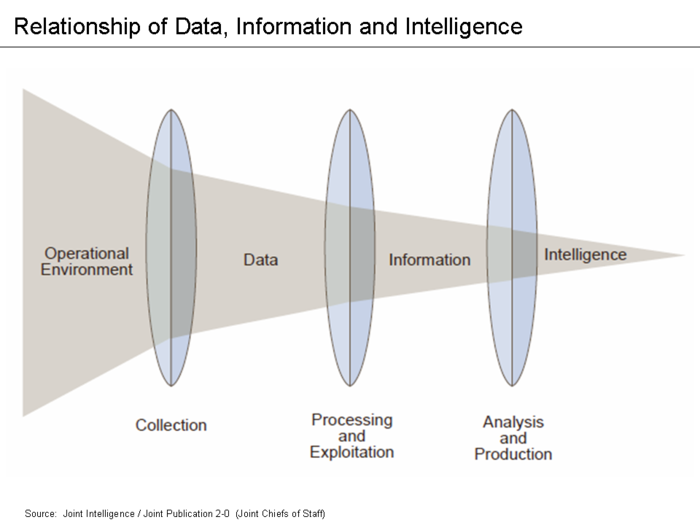
\includegraphics[scale=0.5]{DataAnalysisProcess.png} 
\caption{Here is visible a basic schema of data processes and analysis}
\end{figure}

Data analysis can be divided in some steps:

\begin{enumerate}

% 1
\item Data collection: data can be collected in a variety of ways. For example is possible to collect them using sensors in the environment, such as satellites, recording devices, physical sensors and so on. It is also possible to obtain data through interviews, downloads from online sources, or reading documentation... so the analysis is feasible with a large variety of kinds and sources of data. 

% 2
\item Data processing: raw data must be well-organized for analysis: for example, placing data into row, columns, vector, and so on (but the definition of "well-organized" in this context varies according to the kind of analysis to be performed).

% 3
\item Data cleaning: Once pre-processed and organized, the data may be incomplete, contain duplicates, or contain errors. Data cleaning is the process of correcting these errors, eliminating duplicates and handling incomplete data. Some ways to do this are record matching (comparison between the records to find if there is something suspicious), validation of data (if there is the certainty that data values has to respect some limits), overall evaluation of quality of existing data, de-duplication (process used to remove duplicates). For particular kinds of input this process is very complex (for example vocal input needs an advanced spell-checker), for others is simple (for instance online-survey interviews made using closed choices) 

% 4
\item Exploratory data analysis: in this step the data is analyzed. There are a variety of techniques referred to as "exploratory data analysis", they aim to begin understanding the real content of the data. This process may result in Descriptive statistics, such as the calculation of average or median, or in Data visualization, that allows to examine the data in graphical format, through graphics and other graphical objects.

% 5
\item Modeling and algorithms: another step is using mathematical models to find relations between different variables, such as causality or correlation. An example of this process is the regression analysis.

% 6
\item Communication: this is the final step. It is important to find a way to report the obtained information to the user in an understandable format. The communication must be adapted to the different users, in order to let the data analysis able to meet their requirements.

\end{enumerate}
According to an article written by Andrew Birmingham and Anna Russell (\url{https://which-50.com/this-is-what-big-data-}	\\ \url{really-looks-like-cern-the-universe} 	\url{-and-everything} [4]) in the particular domain of the particles physics this kind of analysis is very important: some experiments at the CERN represents about 150 million sensors delivering data 40 million times per second. There are nearly 600 million collisions per second. This is not the exactly kind of AEgIS experiment, that doesn't generate this gigantic amount of data, but, the point is that not all this information is scientifically interesting. In the huge amount of collisions discussed previously there are only around 100 collisions of interest per second.
This leads a big problem: it is difficult to find a rational way to work with flows of data having this size, and it is strongly required to take only the part of the data actually relevant for the scientific analysis, but it is also important to avoid wasting anything interesting in this dataset.

Another problem to solve to meet the user's requirements is related to the speed with which physicists develop and change focus in their experimental work: they are not interested always at the same things, and they cannot predict in advance what they will need in a remote future, because their needs are related to the process of experimentation, and can change continuously. 
Therefore a system of analysis must be very flexible and dynamic, always ready to serve to new requirements, always able to find exactly what is the "interesting" part of data.  

This kind of problems are not just CERN's problems, they are common in major research centers. Bob Jones, Project Leader at CERN, says:
"CERN is a leader but not alone in having to deal with such high data throughput. We expect to see similar scales in other sciences (such as next generation genome sequencing as well as the Square Kilometer Array which will primarily be deployed in Australia and South Africa) and various business sectors linked to the growing Internet of Things in the near future."
(quote taken from \url{http://www.cloudwatchhub.eu/what-big-data-really}	\\ \url{-looks-cern-universe-and-everything} [4])
 
Big data analysis can provide an answer to this problems: with an intelligent and parametrizable process of filtering it is possible to extract only the subset of scientifically interesting information, and delivering them to the users in an organized and structured way, by tables, statistical values, graphical images. 
In this way is possible to improve the productivity of the physicists, exempting them from unnecessary commitments and dynamically meeting their needs. 


\section{User friendly Data analysis: gAn Web}

GAn is a program that is being used to analyze data related to the AEgIS experiment at CERN, while gAn Web is the web interface to gAn, and it is the main topic of this document.

The goal of gAn Web is to allow users to perform analysis through a more friendly web interface, without install nothing on their machine. In the following image there is a schema that shows how the whole system is organized.

\begin{figure}[H]
\centering
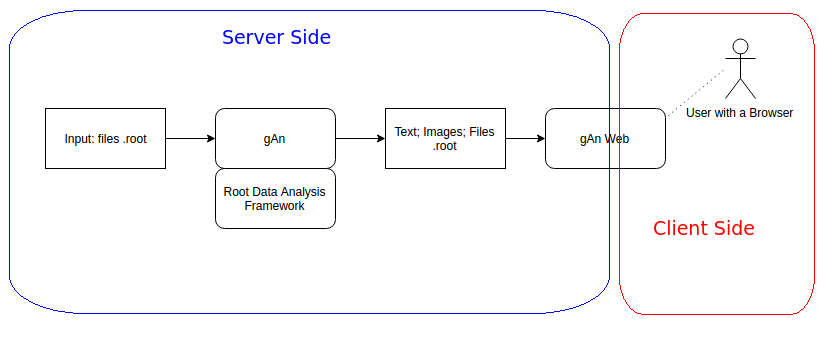
\includegraphics[scale=0.5]{GeneralGAnSchema.png} 
\caption{gAn - gAn Web simple scheme}
\end{figure}

The whole application allows to perform data collection, a process of selection and analysis of data, and data representation. In brief it means being able to extract from a big amount of raw material only the interesting information.

The raw material on which this system works is represented by a set of "Root files". 
The hardware of AEgIS experiment (mostly the sensors) generates these Root files, that are raw, binary files. 
 
The following figure (2.3) presents a schema related to the generation of these input files:

\begin{figure}[H]
\centering
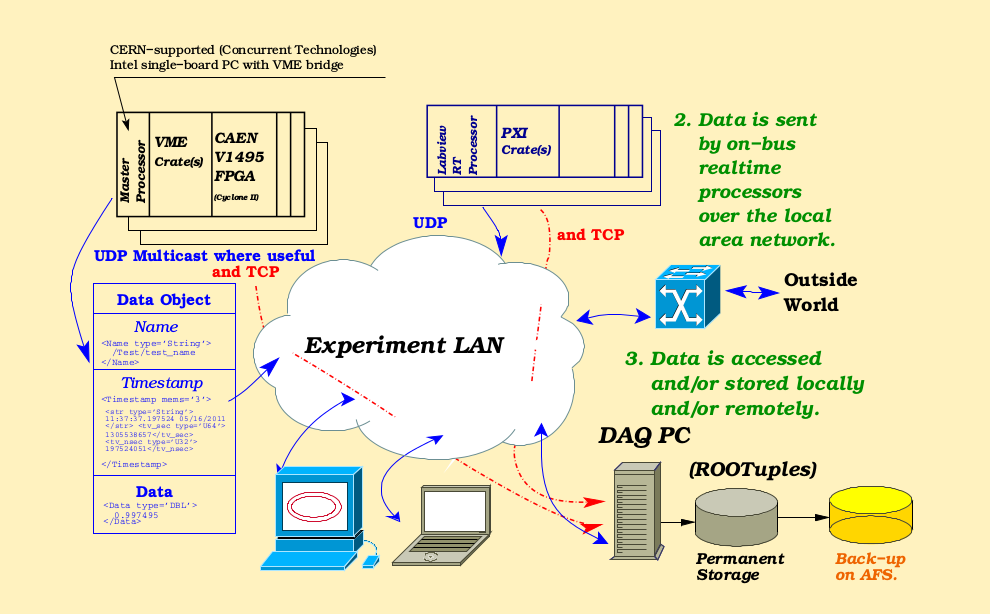
\includegraphics[scale=0.35]{DAQSchema.png} 
\caption{Root format input files generation, DAQ System}
\end{figure}

The data comes from different sensors, that communicate with different protocols, but all the communications use XML as common language. All data are sent through a LAN to a server named DAQ. Here they are stored in the root file to be ready to be analyzed.
The role of DAQ is to cover the first three steps of the data analysis process: it collects, processes and cleans data;

The Root files can be analysed using a framework named ROOT Framework, that consists in a lot of libraries specialized in high-energy physics analysis, and an interpreter able to understand a C++ script.
GAn use this framework, it can access these Root files, make an ordered and organized analysis, extract the most important information, and produce an output that consists of a text with the most important information, comments, and eventual error logs, graphic material such as images of various kind, some other Root format files, with some features used by gAn Web to make further graphical processing, related to the generation of dynamic graphics and figures. 
The goal of gAn is to reduce the big amount of raw data received in input in a little amount of scientifically interesting and easily understandable data in output, covering the forth and the fifth step of the data analysis process: exploratory analysis and modelling and algorithms.

In order to give the correct information gAn require some inputs from the users.

The input parameters inserted by the users are:
\begin{enumerate}

% 1
\item "Run Number", that identifies in which part of the data the user is interested. 
The time in this experiment is divided in "runs" (a run lasts about some hundred seconds), so the user, by the run parameter can tell to gAn in which time slice he is interested. For example: run 55614 means that the user is interested in the information related to the 22th of November 2016, taken in the time slice between 15:45 and 15:47. 
The enumeration of the runs is incremental: so the run 55199 identifies the time slice immediately after the time slices identified by 55198. The progress of the run numbers is always going on, so new run numbers are continuously added. 
In this document every time we say "last run number" we don't mean the absolute last run numbers, but the run number that is going on right in this moment. This concept is important because usually the users use gAn Web on the last existing run number (so on the run number that is going on right at that moment) or on the immediately previous run number.  
This system used to identify time slices seems to be strange at the beginning but is a standard for all the applications in the AEgIS experiment and it allows a very efficient and precise communication. It is indeed a standard in all the experimental activities in high-energy, nuclear and particles physics. This is because inside a "run" there are data related to a specific experimental "configuration".

How can the user have more information about the runs? 
There is a RunLog (sometimes also called LogBook). The RunLog is a document organized by date on which for each run essential and specific information are reported, such as the run number, the date of acquisition, the experimental configuration, and other notes that the physicist that performed the data taking consider important to record.

% 2
\item "Type of analysis", that identifies what gAn must do with the data and what it must show as output to the user.
An analysis is basically a series of operations that treat the data to produce specific output. For example the user can look at the images regarding positrons and antiprotons and calculate the number of particles. Another example is that the user can calculate the fraction of particles that reached the end of the experiment, and so on. Each "analysis" corresponds to a specific source file that gAn loads and run accordingly.

\end{enumerate}


The output of gAn consists of a single text file with computed, (quite) organized data, and a folder of images in png format.
This structure (root files in input, data analysis using Root, images, organized and selected data in output) is very common in the CERN's experiments. 
The output of gAn is quite understandable by an experienced physicist, but it is disorganized, complex for an untrained user, and the terminal interface can be surely improved using some more user friendly technologies.

GAn Web is a web application, that aims to create a user friendly web interface, based on the most important human-machine interaction principles, between the users and gAn. 

A web interface can improve the system in two ways:

\begin{enumerate}

% 1
\item gAn is a stand-alone program based on ROOT, that can be installed on the user's machine; the user has to install the correct version of ROOT to avoid compatibility problems (ROOT is still not perfectly version independent: different versions can occasionally lead to different behaviors). Furthermore, this kind of program is continuously changing, the performed analysis is continuously improved (in the first 2 weeks from the debut of the program there were already several kinds of analysis, because often at the changing of the needs the programmers creates new analysis), so the installed version of gAn is not unchangeable, and the user must often update it. Instead, a centralized version installed on a server, with services accessible from a normal browser by the user can avoid (or at least reduce) this kind of problems and be more usable.    
 

% 2
\item a Linux terminal interface is practical for expert users, but a web based interface can be more attractive for new users, and, if well done, can be easier to use. It is important to notice that all the terminal-based applications exploit the users memory and are prone to errors.


\end{enumerate}



\section{ROOT - Physical Data Analysis }

There are some software (often free software) specialized in the analysis of data. Each of these software has strengths and weaknesses, and none of them appear to be absolutely better than the others. Following there are some examples:
 
\begin{enumerate}

% 1
\item MATLAB (matrix laboratory) is a numerical computing environment. It is a proprietary (t is not available for free, and it is quite expensive) programming language developed by MathWorks. Matlab allows matrix manipulations, plotting of functions and data, implementation of algorithms, creation of user interfaces, and embedding programs written in other languages, including C, C++, Java, Fortran and Python. 
Some detractors say that the statistical support is incomplete if compared with other solutions (also free).

% 2
\item R is a programming language and a software environment for statistical computing. It is supported by the R Foundation for Statistical Computing.The R language is widely diffused for developing statistical software and for data analysis. His popularity has increased in recent years, this is due to the fact that R is free and provides to user a good front-end interface. On the other hand some users say that the learning curve is quite hard at the beginning (in a big research center this is not a big problem..).  

% 3 
\item SciPy/NumPy/Matplotlib are libraries that work in the field of data analysis written for the general purpose language Python. It is a quite immature technology, but it is freely available and it uses a general purpose and widely diffused language like Python.

% 4
\item ROOT is an object-oriented program and library developed by CERN, released the first time in 2003 (the process of development started in 1994 and it has been continuously updated until now). It was originally designed for particle physics data analysis and contains several features specific to this field, but it is also used in other applications such as astronomy and data mining. 

\end{enumerate}

For the AEgIS experiment ROOT is the chosen software to carry out the activities of data analysis. The reason is that this software has been specifically tailored to meet the requirements of the analysis applied to particle physics.
Another advantage of ROOT is that there are a lot of libraries created during the years related to the activities of the experiments of the CERN and it is nearly impossible to rebuild them from scratch with another software.

ROOT development was started by René Brun and Fons Rademakers in 1994 (but a more extended and precise list of collaborators is accessible here \url{https://root.cern.ch/root/htmldoc/guides/users -guide/ROOTUsersGuide.html#preface} [5]). 
The ROOT's user guide start with this prefaction, that explains in detail how ROOT was born:
"In late 1994, we decided to learn and investigate Object Oriented programming and C++ to better judge the suitability of these relatively new techniques for scientific programming. We knew that there is no better way to learn a new programming environment than to use it to write a program that can solve a real problem. After a few weeks, we had our first histogramming package in C++. A few weeks later we had a rewrite of the same package using the, at that time, very new template features of C++. Again, a few weeks later we had another rewrite of the package without templates since we could only compile the version with templates on one single platform using a specific compiler. Finally, after about four months we had a histogramming package that was faster and more efficient than the well-known FORTRAN based HBOOK histogramming package. This gave us enough confidence in the new technologies to decide to continue the development. Thus was born ROOT."
(Taken from \url{https://root.cern.ch/root/htmldoc/guides/users-guide/ROOTUsersGuide.html#preface} [5])


This software is partially released under GPL (this means that everyone is allowed to use, redistribute and change the software, but any changes made must also be licensed under the GPL), and partially under LGPL (The LGPL is similar to the GPL, but is more designed for software libraries in that the developer wants to allow non-GPL applications to link to your library and utilise it).

ROOT is an object oriented framework that aims to solve problems related to high-energy physics. To better understand what is ROOT is important to start with understanding what is a framework: in IT a framework is a structure that helps the programmers providing them a set of already working utilities and services (for example, I/O, graphics, etc.) often related to the sector in which the framework aims to work (for example, the services of a web development framework are related to the layout of a web page, to the organization of DBs etc.). ROOT in particular offers services, functions, and packages related to the world of high-energy physics research, that allow to save much work.
It provides, for example the possibility to use a computer's graphics subsystem and operating system with abstraction, allowing the developer to create a graphical user interface and a GUI builder. ROOT provides also an abstract platform that allows to run C++ and command line scripts. More precisely ROOT includes (among others):

\begin{enumerate}

% 1
\item Libraries related to histogramming and graphing, that allows the developer to easily represent graphically statistical distributions. Also 3D visualization is allowed.

% 2
\item Libraries related to regression analysis.

% 3
\item Various statistics tools. 

% 4
\item Libraries related to digital image processing and manipulation.

% 5
\item Libraries aimed to allow parallel computing, (to parallelize data analysis can be really useful in order to manage the complexity of the calculations).

%6
\item The possibility of interfacing in both directions with code written in Python or Ruby.

%7 
\item The possibility of interfacing with Javascript, allowing the developer to access ROOT functionalities by a Browser.

\end{enumerate}

In the following figure (2.2) we can see the structure of the ROOT's libraries:

\begin{figure}[H]
\centering
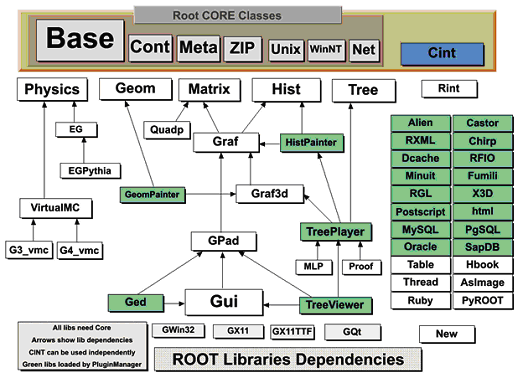
\includegraphics[scale=0.5]{RootStructure.png} 
\caption{ROOT structure}
\end{figure}


